% --- To be compiled with XeLaTeX ---
% ---      Encoding: UTF-8        ---

\documentclass[a4paper, oneside, 11pt]{article}

%fontspec package provides a configurable interface for font selection, and allows complex font choices to be named and later reused. It's needed for XeLaTeX
\usepackage[cm-default]{fontspec}

% Unicode support
\usepackage{xunicode}
\usepackage{xltxtra}

% Default words and phrases in Greek (e.g. 'Περίληψη' instead of 'Abstract'). Also contains hyphenation rules for Greek Language
\usepackage{xgreek}

% Mathematical fonts, theorems etc.
\usepackage{amsfonts}
\usepackage{amsmath}
\usepackage{amsthm}

% Default page layout for consuming a larger portion of the page.
\usepackage{fullpage}

% Greek fonts (Computer Modern)
\setmainfont[Mapping=tex-text]{CMU Serif}

% Auxiliary commands
\newcommand{\red}{\leq_{\text{m}}}

\newtheorem{thm}{Θεώρημα}
\newtheorem{lm}[thm]{Λήμμα}

\theoremstyle{definition}
\newtheorem{defn}[thm]{Ορισμός}

\begin{document}

% Auxiliary commands
\newcommand{\HRule}{\rule{\linewidth}{0.5mm}}

\begin{titlepage}
\begin{center}


\includegraphics[width=0.3\textwidth]{../logos/pyrforos.png}
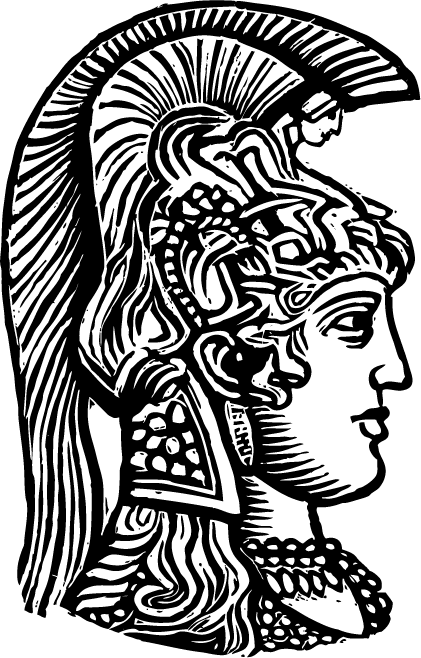
\includegraphics[width=0.2\textwidth]{../logos/uoa.png}\\[1cm]

\textsc{\LARGE Σχολή Ηλεκτρολόγων Μηχανικών και Μηχανικών Υπολογιστών}\\[1.5cm]

\HRule \\[0.4cm]
{\huge \bfseries Υπολογισιμότητα\\
\LARGE Ομάδα Ασκήσεων No. 2}\\[0.4cm]

\HRule \\[1.5cm]

\begin{center}
\textbf{Ομάδα}\\
Αξιώτης Κυριάκος\\
Αρσένης Γεράσιμος
\end{center}

\vfill

{\large \today}
\end{center}

\end{titlepage}


\section*{Άσκηση 1}

\begin{itemize}
   \item \textbf{Ψευδής}
   
         Έστω $x$ τέτοιο ώστε $M_x$ να είναι μια TM η οποία δεν τερματίζει για καμία
         είσοδο.  Τότε έχουμε $\text{Dom}(\phi_x) = \emptyset$ το οποίο είναι
         αναδρομικό σύνολο (το αποφασίζει η μηχανή Turing που απορρίπτει κάθε
         είσοδο), δηλαδή $x \in R$. Όμως από τον ορισμό της $M_x$ έχουμε $M_x(x)
         \uparrow$, δηλαδή $x \notin K$.

   \item \textbf{Ψευδής}

         Έστω $x$ τέτοιο ώστε $M_x$ να είναι μια TM η οποία τερματίζει και
         αποδέχεται κάθε είσοδο.
         Τότε έχουμε $\text{Dom}(\phi_x) = \mathbb{N}$ το οποίο είναι
         αναδρομικό σύνολο (το αποφασίζει η μηχανή Turing που αποδέχεται κάθε
         είσοδο), δηλαδή $x \in R$. Όμως από τον ορισμό της $M_x$ έχουμε $M_x(x)
         \downarrow$, δηλαδή $x \in K$ συνεπώς $x \in R \cap K$.

   \item \textbf{Ψευδής}

         Στα παρακάτω θα χρησιμοποιήσουμε το εξής πρόβλημα:

         \[ \text{HALT} = \{ \langle M, w \rangle\ |\ M(w) \downarrow \} \]

         για το οποίο γνωρίζουμε ότι $\text{HALT } \in \text{ ER}$ και
         $\text{HALT } \notin \text{REC}$ επομένως
         $\overline{\text{HALT} } \notin \text{ ER}$ και θα κάνουμε την
         αναγωγή $\overline{\text{HALT} } \red R$ από την οποία
         προκύπτει ότι $R \notin \text{ER}$. Συνεπώς και $R \cup K \notin \text{ER}$.

         \begin{lm}
            $\overline{\text{HALT}} \red R$.
         \end{lm}
         \begin{proof}
            Θα πρέπει να βρούμε μια συνάρτηση $f : \mathbb{N} \rightarrow \mathbb{N}$
            η οποία να είναι υπολογίσιμη και για την οποία
            να ισχύει:
            $\langle M, w \rangle \in \overline{\text{HALT}} \Leftrightarrow
               f(\langle M, w \rangle) \in R$.

            Αυτή η $f$ θα είναι η συνάρτηση που υπολογίζει η παρακάτω μηχανή Turing:

            \begin{itemize}
               \item $F = $`` Για είσοδο $\langle M, w \rangle$:
               \begin{enumerate}
               \item Δημιούργησε την περιγραφή και βρες
                     τον αριθμό G\"{o}del $g$ της μηχανής Turing $T$:\\
                     $T = $ `Για είσοδο $\langle T_1, x \rangle$:
                     \begin{enumerate}
                     \item Προσομοίωσε παράλληλα την $M$ με είσοδο $w$ και
                           την $T_1$ με είσοδο $x$.
                     \item Αν τερματίσουν και οι δύο, τότε επέστρεψε το $T_1(x)$.'
                     \end{enumerate}
               \item Γράψε $g$ στην ταινία εξόδου.''
               \end{enumerate}
            \end{itemize}

            Έστω ότι $\langle M, w \rangle \in \overline{\text{HALT}}$, δηλαδή $M(w)
            \uparrow$, τότε η μηχανή $T$ δεν τερματίζει για καμία είσοδο άρα
            $f(\langle M, w \rangle) = g$ όπου $g$ τέτοιο ώστε $\text{Dom}(\phi_g) =
            \emptyset \in \text{REC}$, συνεπώς $g \in R$.

            Αντίστροφα, αν $\langle M, w \rangle \in \text{HALT}$ τότε η συνάρτηση $f$
            επιστρέφει ένα $g$ για το οποίο $\text{Dom}(\phi_g) = \text{HALT} \notin
            \text{REC}$, άρα $g \in \overline{R}$.
         \end{proof}
         
\end{itemize}

\section*{Άσκηση 2}

\begin{lm}
Το πρόβλημα ΔΙΑΨΕΥΣΗ GOLDBACH είναι αναγνωρίσιμο.
\end{lm}
\begin{proof}
Θεωρούμε τη μηχανή Turing με την εξής λειτουργία: Αν $n$ είναι η είσοδος της μηχανής,
δοκιμάζει με τη σειρά τους ακεραίους $k\geq n$. Για κάθε τέτοιο αριθμό, δοκιμάζει όλα
τα ζευγάρια ακεραίων $p,q\leq 2k$, τα οποία προφανώς είναι πεπερασμένα για σταθερό $k$,
και ελέγχει αν τα $p$ και $q$ είναι πρώτοι (δοκιμάζοντας όλους τους πιθανούς διαιρέτες)
και αν $2k = p + q$. Αν για κάποιο $k$ δεν βρεθούν $p$ και $q$ που να ικανοποιούν τις
παραπάνω ιδιότητες, τότε η μηχανή Turing απαντάει ΝΑΙ στο πρόβλημα ΔΙΑΨΕΥΣΗ GOLDBACH.
Πραγματικά, αν υπάρχει ακέραιος $k\geq n$ που να διαψεύδει την εικασία του Goldbach,
τότε δεν θα υπάρχει ζευγάρι πρώτων $p,q\leq 2k$ έτσι ώστε $2k = p+q$. Η μηχανή Turing
θα φτάσει σε αυτό το $k$ σε πεπερασμένο χρόνο, άρα σε πεπερασμένο χρόνο θα απαντήσει
ΝΑΙ. Συνεπώς το πρόβλημα ΔΙΑΨΕΥΣΗ GOLDBACH είναι αναγνωρίσιμο.
\end{proof}

\begin{lm}
Αν το πρόβλημα ΕΠΑΛΗΘΕΥΣΗ GOLDBACH είναι αναγνωρίσιμο, τότε θα είναι και διαγνώσιμο.
\end{lm}
\begin{proof}
Θεωρούμε τη μηχανή Turing $M_1$, η οποία αναγνωρίζει το πρόβλημα ΕΠΑΛΗΘΕΥΣΗ GOLDBACH,
και τη μηχανη $M_2$, η οποία αναγνωρίζει το πρόβλημα ΔΙΑΨΕΥΣΗ GOLDBACH. Τώρα, έστω
μηχανή $M$ η οποία εξομοιώνει τις μηχανές $M_1$ και $M_2$ για ένα βήμα την
καθεμιά εναλλάξ. Αν κάποια στιγμή αποδεχθεί η $M_1$, τότε η $M$ τερματίζει και δίνει
απάντηση ΝΑΙ για το πρόβλημα ΕΠΑΛΗΘΕΥΣΗ GOLDBACH. Αν, από την άλλη, κάποια στιγμή
αποδεχθεί η $M_2$, τότε η $M$ τερματίζει και δίνει απάντηση ΟΧΙ για το πρόβλημα 
ΕΠΑΛΗΘΕΥΣΗ GOLDBACH. Επειδή κάποιο από τα δύο παραπάνω σενάρια θα συμβεί σε πεπερασμένο
χρόνο, η μηχανή $M$ τερματίζει σε πεπερασμένο χρόνο και αποφασίζει το πρόβλημα
ΕΠΑΛΗΘΕΥΣΗ GOLDBACH. Αυτό σημαίνει ότι το πρόβλημα αυτό είναι διαγνώσιμο.
\end{proof}

\section*{Άσκηση 3}

Όπως έχουμε δεί και στο μάθημα, αν μια μηχανή Turing είναι περιορισμένη στις πρώτες
$n$ θέσεις τότε υπάρχουν $t(n) = |Q| \cdot n \cdot |\Sigma|^n$ πιθανές καταστάσεις στις
οποίες μπορεί να βρίσκεται κάθε στιγμή. Αν βρεθεί σε κάποια από αυτές τις καταστάσεις
για δεύτερη φορά τότε θα πέσει σε άπειρο βρόχο.

Επομένως για μια μή περιορισμένη TM, ο μόνος τρόπος να φτάσει στη θέση $n+1$ είναι να
το κάνει σε λιγότερο από $t$ βήματα.

Φτιάχνουμε λοιπόν μια μηχανή Turing T η οποία για είσοδο $\langle M, w, n_1, n_2
\rangle$ προσομοιώνει την $M$ με είσοδο $w$ για $t(\min(n_1, n_2)-1)$ βήματα και αν η
$M$ φτάσει στη θέση $\min(n_1, n_2)$ αποδέχεται διαφορετικά απορρίπτει.

Η T αποφασίζει το πρόβλημα ΠΕΠΕΡΑΣΜΕΝΗ ΜΝΗΜΗ αφού πάντα τερματίζει και αποδέχεται ανν
η $M$ επισκεφτεί την θέση $\min(n_1, n_2)$ το οποίο είναι ισοδύναμο με το να
επισκεφτεί κάποια εκ των θέσεων $n_1, n_2$ αφού για να πάει μια μηχανή Turing από μία
θέση σε μία άλλη θα πρέπει να περάσει από όλες τις ενδιάμεσες.

\section*{Άσκηση 4}

Έστω οποιαδήποτε μηχανή Turing $M_1$ και είσοδος $x$. Θα δείξουμε ότι αν η γλώσσα $L$ ήταν αναδρομική,
τότε θα μπορούσαμε να ξέρουμε σε πεπερασμένο χρόνο αν η $M_1$ με είσοδο $x$ τερματίζει ή όχι.
Έστω $M$ μηχανή Turing που αποφασίζει τη γλώσσα $L$. Θα κατασκευάσουμε μία μηχανή $M_2$, η οποία θα είναι
ίδια με την $M_1$, με τη διαφορά ότι για κάθε μετάβαση από μία κατάσταση $q$ σε μία τελική κατάσταση $q'$ 
με τον κανόνα $(q',\gamma_1',m)=\delta_1(q,\gamma)$, για κάποιο σύμβολο $\gamma$, θα αλλάξουμε τη συνάρτηση
μετάβασης σε $(q',\gamma_2',m)=\delta_2(q,\gamma)$, όπου $\gamma_1'\neq \gamma_2'$. Δηλαδή απλώς θα αλλάξουμε το σύμβολο που γράφεται
στην ταινία πριν από μια τελική κατάσταση.
\begin{lm}
Η $M_1$ δεν τερματίζει με είσοδο $x$ αν και μόνο αν οι $M_1$ και $M_2$ κατά τη λειτουργία τους με είσοδο
$x$ γράφουν μετά από τον ίδιο αριθμό βημάτων το ίδιο σύμβολο στην ταινία τους.
\end{lm}
\begin{proof}
Αν η $M_1$ δεν τερματίσει, τότε δεν θα βρεθεί ποτέ σε τελική κατάσταση, άρα οι $M_1$ και $M_2$ θα έχουν 
πανομοιότυπη λειτουργία.
Από την άλλη, αν τερματίσει, αυτό σημαίνει ότι το τελευταίο σύμβολο που θα γράψει η $M_1$ θα είναι 
διαφορετικό από το σύμβολο που θα γράψει η $M_2$ μετά από τον ίδιο αριθμό βημάτων.
\end{proof}

\section*{Άσκηση 5}

\begin{lm}
$L \in \text{ER}$
\end{lm}
\begin{proof}
Μπορούμε να απαριθμήσουμε τα στοιχεία της $L$ με τον εξής απαριθμητή:

$T = $``Για κάθε $k \in \mathbb{N}$ προσομοίωσε κάθε μηχανή Turing $M_i$ με $1 \leq i
\leq k$ για $k-i+1$ βήματα αντίστοιχα για κάθε μία από τις $|\Sigma|^{2013}$ πιθανές
εισόδους $x$ για τις οποίες $|x| = 2013$. Αν κάποια από αυτές τις μηχανές αποδεχτεί
την είσοδό της τότε τυπωσε τον αριθμό G\"{o}del της.''

Αν υπάρχει $x \in \Sigma^*$ με $|x| = 2013$ το οποίο να το αποδέχεται η $M_i$ σε $m$
βήματα τότε ο απαριθμητής θα τυπώσει το $\langle M_i \rangle$ όταν $k = i+m$ το οποίο
θα συμβεί σε πεπερασμένο πλήθος βημάτων.
\end{proof}

\begin{lm}
$\overline{L} \notin \text{ER}$
\end{lm}
\begin{proof}
Θα δείξουμε ότι $L \notin \text{REC}$ από το οποίο προκύπτει ότι $\overline{L} \notin
ER$.

Έστω ότι η $L$ ήταν αποφάνσιμη και έστω $R$ μια TM που αποφασίζει την $L$.
Τότε θα μπορούσαμε να δημιουργήσουμε την εξής TM που αποφασίζει το πρόβλημα HALT (βλ.
Άσκηση 1).

\begin{itemize}
\item $T = $``Για είσοδο $\langle M, w \rangle$:
      \begin{enumerate}
      \item Δημιούργησε την περιγραφή και βρες τον αριθμό G\"{o}del $g$ της μηχανής
      Turing που αγνοεί την είσοδό της, προσομοιώνει την $M$ για είσοδο $w$.
      και αποδέχεται ανν η $M$ τερματίσει.
      \item Προσομοίωσε την $R$ με είσοδο $g$ και απάντησε accept ανν η $R$
      αποδεχθεί.''
      \end{enumerate}
\end{itemize}

Η $T$ πάντα τερματίζει αφού υποθέσαμε ότι και η $R$ πάντα τερματίζει και αποδέχεται
την είσοδο $\langle M, w \rangle$ ανν $M(w) \downarrow$, δηλαδή η $T$ αποφασίζει το
HALT. Άτοπο, άρα $L \notin \text{REC}$.
\end{proof}

\section*{Άσκηση 6}

Προφανώς η γλώσσα των παλινδρόμων είναι αναδρομική, αφού μπορούμε σε πεπερασμένο χρόνο να αναποδογυρίσουμε
μία συμβολοσειρά και να ελέγξουμε αν είναι ίση με την αρχική. Έστω $M_1$ η μηχανή Turing που αποφασίζει
αυτή την γλώσσα.
Έστω τώρα μία αναγνωρίσιμη γλώσσα $L$ και $M_2$ μηχανή Turing που την αναγνωρίζει. 
Θεωρούμε μία μηχανή Turing $Μ$ και είσοδο $x$, η οποία πρώτα εξομοιώνει την $M_1$ με είσοδο $x$. 
Αν η $M_1$ δεν αποδεχθεί
την $χ$, τότε η $M$ τρέχει για πάντα. Αλλιώς, η $M$ εξομοιώνει την $M_2$ με είσοδο και αν αυτή αποδεχθεί,
αποδέχεται και η $M$. Αλλιώς, τρέχει για πάντα. Προφανώς, για να αποδεχθεί η $M$ πρέπει η $x$ να είναι
και παλίνδρομο, αλλά και να ανήκει στη γλώσσα $L$. Αντίστροφα, αν η $x$ είναι παλίνδρομο και ανήκει στην $L$
τότε θα την αποδεχθούν και η $M_1$ και η $M_2$. Συνεπώς το σύνολο των παλινδρόμων της $L$ είναι αναγνωρίσιμο.

\section*{Άσκηση 7}

Θα δείξουμε ότι $\overline{\text{HALT}} \red L$ και συνεπώς $L \notin \text{ER}$ αφού
$\overline{\text{HALT}} \notin \text{ER}$.

Η συνάρτηση $f$ της αναγωγής υπολογίζεται από την παρακάτω TM:

\begin{itemize}
\item $T = $``Για είσοδο $\langle M, w \rangle$:
      \begin{enumerate}
      \item Δημιούργησε τις μηχανές Turing:
            \begin{enumerate}
               \item $M_1(x) = $`Αγνόησε την είσοδο και πέσε σε άπειρο βρόχο.'
               \item $M_2(x) = $`Αγνόησε την είσοδο, προσομοίωσε την $M$ με είσοδο $w$ και
               τερμάτισε ανν $M(w) \downarrow$.'
            \end{enumerate}
      \item Επέστρεψε $\langle M_1, M_2 \rangle$.''
      \end{enumerate}
\end{itemize}

Αν $\langle M, w \rangle \in \overline{\text{HALT}}$, δηλαδή $M(w) \uparrow$ τότε
για κάθε $x \in \Sigma^*: M_2(x) \uparrow$ άρα $\langle M_1, M_2 \rangle \in L$.
Αντίστροφα, αν $\langle M, w \rangle \in \text{HALT}$, τότε για κάθε $x: M_2(x)
\downarrow$. Επίσης εξ ορισμού για κάθε $x: M_1(x) \uparrow$ συνεπώς $\langle
M_1, M_2, \rangle \in \overline{L}$.

\section*{Άσκηση 8}

(Θεωρούμε ότι ο τελεστής $\lfloor\cdot\rfloor$ είναι ο αντίστροφος του $\langle\cdot\rangle$.)

\begin{defn}
Ορίζουμε ως \textit{άχρηστες} καταστάσεις μιας μηχανής Turing, αυτές προς τις οποίες δεν υπάρχει καμία
μετάβαση στον πίνακα μεταβάσεων από άλλες καταστάσεις, 
και ούτε είναι αρχικές καταστάσεις. Επίσης ορίζουμε $u(\langle M\rangle)$ 
το πλήθος των άχρηστων καταστάσεων της μηχανής Turing $M$. Η συνάρτηση $u$ είναι υπολογίσιμη, αφού μια μηχανή
Turing $M'$ μπορεί να πάρει την κωδικοποίηση της $M$ και να μετρήσει πόσες καταστάσεις δεν εμφανίζονται στον
πίνακα μεταβάσεων και ούτε είναι αρχικές.
\end{defn}


Έστω τώρα μηχανή Turing $\widetilde{M}^x$ και είσοδος $y$ σε αυτήν, όπου $x$ και $y$ κωδικοποιήσεις μηχανών
Turing. Θα περιγράψουμε τη λειτουργία της.
Αρχικά, η $\widetilde{M}^x$ υπολογίζει το πλήθος των άχρηστων καταστάσεων $u(y)$ της μηχανής $\lfloor y\rfloor$.
Στη συνέχεια, εξομοιώνει τη μηχανή $\lfloor x\rfloor$ με είσοδο $u(y)$. Αν η τελευταία τερματίσει, τότε και η
$\widetilde{M}^x$ τερματίζει και αποδέχεται. Θεωρούμε ότι η
$\widetilde{M}^x$ δεν έχει άχρηστες καταστάσεις.

Τώρα, ορίζουμε για κάθε φυσικό $i$, τη μηχανή Turing $\widetilde{M}_i^x$, η οποία είναι η $\widetilde{M}^x$
με επιπλέον $i$ άχρηστες καταστάσεις. Προφανώς, αυτή μπορεί να κατασκευαστεί σε πεπερασμένο
χρόνο.

\begin{lm}
Έστω μηχανή Turing $M$ που αναγνωρίζει κάποιο αναδρομικά απαριθμήσιμο πρόβλημα και είσοδος $x$ σε αυτήν. 
Η $M(x)$ έχει το ίδιο αποτέλεσμα (αποδοχή ή μη τερματισμός) με την
$\widetilde{M}_x^{\langle M\rangle}(\langle\widetilde{M}_x^{\langle M\rangle}\rangle)$.
\end{lm}
\begin{proof}
Εκ κατασκευής, έχουμε ότι $u(\langle\widetilde{M}_x^{\langle M\rangle}\rangle)=x$. Άρα το αποτέλεσμα
της $\widetilde{M}_x^{\langle M\rangle}(\langle\widetilde{M}_x^{\langle M\rangle}\rangle)$ είναι το ίδιο με το
αποτέλεσμα της $M(u(\langle\widetilde{M}_x^{\langle M\rangle}\rangle))$, το οποίο 
είναι με τη σειρά του ίδιο με αυτό της $M(x)$.
\end{proof}

Από τα παραπάνω συμπεραίνουμε ότι υπάρχει απεικονιστική αναγωγή από κάθε αναδρομικά απαριθμήσιμο πρόβλημα
στο $K=\{\langle M\rangle | M(\langle M\rangle)\downarrow\}$.

\section*{Άσκηση 9}

Έστω $T_1, T_2$ οι μηχανές που αναγνωρίζουν τις γλώσσες $\overline{A}, \overline{B}$
αντίστοιχα.

Δημιουργούμε την μηχανή $T$:

\begin{itemize}
\item $T = $`` Για είσοδο $x$:
      \begin{enumerate}
         \item Τρέξε παράλληλα την $T_1$ με είσοδο $x$ και την $T_2$ με είσοδο $x$
               μέχρι κάποια εκ των δύο να τερματίσει.
         \item Αν τερμάτισε η $T_1$ τότε επέστρεψε $\overline{T_1(x)}$.
         \item Αν τερμάτισε η $T_2$ τότε επέστρεψε $T_2(x)$.''
      \end{enumerate}
\end{itemize}

Θα δείξουμε ότι $C = L(T)$ είναι η γλώσσα που αναζητούμε.

Αρχικά παρατηρούμε ότι η $T$ πάντα τερματίζει αφού $A \cap B = \emptyset
\Leftrightarrow \overline{A} \cup \overline{B} = \Sigma^*$. Άρα για κάθε $x \in
\Sigma^*$, έχουμε είτε $x \in \overline{A}$ είτε $x \in \overline{B}$ συνεπώς μία εκ
των $T_1, T_2$ θα αποδεχτεί το $x$ κι έτσι $C \in \text{REC}$.

\begin{itemize}
\item $A \subseteq C$:
      
      Έστω $x \in A$. Αφού $A \cap B = \emptyset$ θα έχουμε $x \notin B
      \Rightarrow x \in \overline{B}$.

      Εκτελούμε τη μηχανή $T$ με είσοδο το $x$. Επειδή $x \in \overline{B}$ ξέρουμε
      ότι η $T_2$ θα τερματίσει κάποια πεπερασμένη χρονική στιγμή και θα αποδεχτεί.
      Αν τερματίσει πριν την $T_1$ τότε θα εκτελεστεί η γραμμή 3 και έτσι και η $T$
      αποδέχεται. Διαφορετικά, αν η $T_1$ τερματίσει πρώτη θα
      πρέπει αναγκαστικά να απαντήσει reject, συνεπώς λόγω της γραμμής 2 η $T$ θα
      αποδεχθεί.

      Σε κάθε περίπτωση η $T$ αποδέχεται το $x$, συνεπώς $x \in C$.

\item $B \subseteq \overline{C}$

      Έστω $x \in B$. Αντίστοιχα με προηγουμένως εκτελούμε την $T$ με είσοδο $x$ και
      επειδή $x \notin A$ η $T_1$ θα αποδεχτεί σε πεπερασμένο πλήθος βημάτων. Αν η
      $T_1$ τερματίσει πρώτη τότε η $T$ απορρίπτει ενώ αν η $T_2$ τερματίσει πρώτη
      αναγκαστικά θα απορρίψει και έτσι και η $T$ θα απορρίψει.

      Σε κάθε περίπτωση $x \notin C$.
\end{itemize}

\section*{Άσκηση 10}

Έστω $S$ μη κενό υποσύνολο του $\mathbb{N}$ που είναι αναδρομική γλώσσα. Θα δείξουμε
ότι οποιαδήποτε πλήρης αύξουσα συνάρτηση $f$ με πεδίο τιμών το $S$ είναι αναδρομική.
Έστω ότι το $S$ είναι πεπερασμένο και $S=\{a_1,a_2,...,a_n\}$ με $a_1 < a_2 < ... < a_n$.
Τότε, θα υπάρχουν θετικοί ακέραιοι $c_1 < c_2 < ... < c_{n-1}$, έτσι ώστε 
$f(1)=f(2)=...=f(c_1)=a_1$, $f(c_1+1)=f(c_1+2)=...=f(c_2)=a_2$, ..., 
$f(c_{n-2}+1)=...=f(c_{n-1})=a_{n-1}$ και $f(x)=a_n$ για κάθε $x>c_{n-1}$. Κάθε τέτοια
συνάρτηση είναι προφανώς αναδρομική, αφού κάποια μηχανή Turing μπορεί απλώς να ελέγξει
σε ποιο από τα διαστήματα $[c_i+1,c_{i+1}]$ βρίσκεται η είσοδος και να επιστρέψει
την τιμή που αντιστοιχεί σε αυτό (Θεωρούμε $c_0=0$ και $c_n=\infty$).
Έστω τώρα ότι το $S$ είναι άπειρο και $S=\{a_1,a_2,...,a_n,...\}$ με 
$a_1<a_2<...<a_n<...$. Τότε, θα υπάρχουν θετικοί ακέραιοι $c_1 < c_2 < ... < c_n < ...$,
έτσι ώστε $f(1)=f(2)=...=f(c_1)=a_1, f(c_1+1)=...=f(c_2)=a_2, ... , f(c_{n-1}+1)=...=f(c_{n})=a_n = ...$.
Άρα, και εδώ, για τον ίδιο λόγο με την προηγούμενη περίπτωση, η $f$ είναι αναδρομική.

Αντίστροφα τώρα, έστω πλήρης αύξουσα και αναδρομική συνάρτηση $f$ με πεδίο ορισμού $S$
υποσύνολο του $\mathbb{N}$. Θα δείξουμε ότι το $S$ είναι αναδρομικό.
Έστω είσοδος $x$. 
Αν το $S$ είναι πεπερασμένο, τότε προφανώς είναι και αναδρομικό, αφού μια μηχανη Turing
μπορεί να ελέγξει αν το $x$ είναι ένα από τα (πεπερασμένα σε πλήθος) στοιχεία του $S$
ή όχι σε πεπερασμένο χρόνο. Αν τώρα το $S$ είναι άπειρο, τότε θα υπάρχει $t$ έτσι
ώστε $f(t) \geq x$. Έστω το ελάχιστο τέτοιο $t$. Αυτό είναι πεπερασμένο, άρα μπορούμε
να το υπολογίσουμε. Τώρα, αν $f(t) > x$ έχουμε ότι $x\notin S$, ενώ αν $f(t) = x$
έχουμε ότι $x\in S$. Συνεπώς το $S$ είναι αναδρομικό.

\section*{Άσκηση 11}

Έστω $L$ μια άπειρη αναδρομικά απαριθμήσιμη γλώσσα. Συνεπώς υπάρχει ένας απαριθμητής
$T$ ο οποίος τυπώνει στην έξοδό του όλες τις λέξεις της γλώσσας με αυθαίρετη σειρά
και πιθανόν με επαναλήψεις.

Αρχικά παρατηρούμε ότι μπορούμε να δημιουργήσουμε μια μηχανή $T'$ παρόμοια με την $T$
με τη διαφορά ότι θα διατηρεί μια λίστα με τις λέξεις που έχει τυπώσει και πριν
τυπώσει μια λέξη να ελέγχει ότι όντως είναι η πρώτη φορά που την τυπώνει. H $T'$
συνεχίζει να είναι απαριθμητής της $L$ αφού αν η $T$ τύπωνε μία λέξη $w$ σε
πεπερασμένο αριθμό βημάτων το ίδιο θα κάνει και η $T'$.

Άρα θεωρούμε χωρίς βλάβη της γενικότητας ότι η $T$ τυπώνει κάθε λέξη της $L$ ακριβώς
μία φορά οπότε δημιουργούμε τις μηχανές $T_1, T_2$ οι οποίες κάνουν ό,τι κάνει και η
$T$ με τη διαφορά ότι τυπώνουν κάθε δεύτερη λέξη ξεκινώντας από την πρώτη ή τη
δεύτερη αντίστοιχα.

Άρα οι $T_1, T_2$ απαριθμούν τις άπειρες γλώσσες $A, B$ για τις οποίες $A \cap B =
\emptyset$ και $A \cup B = L$.

\section*{Άσκηση 12}

Έστω σταθερό $x\in \mathbb{N}$. Για οποιοδήποτε $y\in \mathbb{N}$ με $y\leq x$ έχουμε
ότι $y\in Im(\phi_{f(x)})$ αν και μόνο αν $\phi_y(y)\downarrow$. Δεν υπάρχει τίποτα 
άλλο στο $Im(\phi_{f(x)})$. Θεωρούμε την εξής μηχανή Τuring $M$ με είσοδο $y$:
Αν $y\leq x$ και $\phi_y(y)\downarrow$, η $M$ τερματίζει και επιστρέφει $y$. 
Διαφορετικά, η $M$ τρέχει για πάντα. 
Παρατηρούμε ότι αφού τα $y\leq x$ είναι πεπερασμένα, η $M$ δεν χρειάζεται να ελέγξει
αν $\phi_y(y)\downarrow$. Μας αρκεί ότι θα \textit{υπάρχει} μια τέτοια $M$. Αυτό φαίνεται
πιο εύκολα αν θεωρήσουμε όλες τις $2^{x+1}$ δυνατές μηχανές Turing, ανάλογα με το αν 
τερματίζουν ή δεν τερματίζουν σε κάθε $y\leq x$. Kάποια από αυτές είναι η $M$.
Συνεπώς $Im(\phi_{f(x)})\in REC$. Παρατηρούμε ότι αν μπορούσαμε κατασκευαστικά να βρούμε τη μηχανή Turing $M$, τότε θα μπορούσαμε να αποφασίσουμε τη γλώσσα της άσκησης 8, η οποία όμως είναι μη αποφάνσιμη.

%Λάθος.
%Αν ίσχυε το ζητούμενο, τότε για $x,y\in \mathbb{N}$ με $x=y$
%θα μπορούσαμε να αποφασίσουμε εάν $x\in Im(\phi_{f(x)})$, δηλαδή αν
%$\phi_x(x)\downarrow$ ή $\phi_x(x)\uparrow$. Έστω $M_i$ αρίθμηση όλων των μηχανών Turing
%έτσι ώστε η $M_i$ να υπολογίζει τη συνάρτηση $\phi_i$. Αυτό σημαίνει ότι για κάθε $i$,
%μπορούμε να αποφασίσουμε αν το $M_i(i)$ τερματίζει ή όχι. Αν θεωρήσουμε $\langle M_i\rangle=i$,
%λοιπόν, για κάθε μηχανή Turing $M$ μπορούμε να αποφασίσουμε αν το $M(\langle M\rangle)$ τερματίζει
%ή όχι. Αυτό έρχεται σε ευθεία αντίθεση με την άσκηση 8, στην οποία δείξαμε ότι το πρόβλημα
%$K=\{\langle M\rangle | M(\langle M\rangle) \downarrow\}$ είναι ER-πλήρες, δηλαδή ότι το
%πρόβλημα τερματισμού ανάγεται σε αυτό. Άρα το $K$ δεν είναι αναδρομικό, και συνεπώς υπάρχουν
%άπειρα $x$ για το οποία το $Im(\phi_{f(x)})$ δεν είναι αναδρομικό. Επίσης αν για κάποιο
%$x$ το $Im(\phi_{f(x)})$ είναι αναδρομικό, τότε και για όλα τα $y<x$ το $Im(\phi_{f(y)})$
%είναι αναδρομικό, άρα το $Im(\phi_{f(x)})$ είναι αναδρομικό μόνο για πεπερασμένο πλήθος
%διαφορετικών $x$.

\section*{Άσκηση 13}

Έστω η ΤΜ:

\begin{itemize}
\item $T = $``Για είσοδο $n$:
      \begin{enumerate}
      \item Για $1 \leq i \leq n$:
            \begin{enumerate}
            \item Προσομοίωσε την $M_i$ με είσοδο $n$ και τοποθέτησε το αποτέλεσμα σε
                  μία ειδική ταινία.
            \end{enumerate}
      \item Υπολόγισε και επέστρεψε το άθροισμα όλων των τιμών της ειδικής ταινίας.''
      \end{enumerate}
\end{itemize}

Θα δείξουμε ότι η $T$ υπολογίζει την $f$. Πράγματι, αν για κάποιο $n$ η $f$ ορίζεται,
δηλαδή ισχύει
$n \in \text{Dom}(\phi_i)$ για κάθε $1 \leq i \leq n$ τότε η 
κάθε προσομοίωση στο βήμα 1 τερματίζει μετά από πεπερασμένο αριθμό βημάτων και έτσι η
$T$ τερματίζει και επιστρέφει $T(n) = f(n)$

\section*{Άσκηση 14}

Έστω $L$ αναδρομικά απαριθμήσιμη γλώσσα. Θα δείξουμε ότι υπάρχει επί, πλήρης και υπολογίσιμη
συνάρτηση $f:\mathbb{N}\rightarrow L$. Θεωρούμε μηχανή Turing $M$ που αναγνωρίζει την $L$.
Τρέχουμε την $M$ για όλες τις δυνατές εισόδους με dovetailing, έτσι ώστε κάθε είσοδος να εμφανίζεται
άπειρο αριθμό φορών. Έστω $x_0, x_1, ... $ η άπειρη
ακολουθία (όχι διακριτών) εισόδων για τις οποίες η $M$ αποδέχεται. Εφόσον η $L$ είναι
αναδρομικά απαριθμήσιμη, για κάθε $x\in L$ υπάρχει $i\in \mathbb{N}$ έτσι ώστε $x=x_i$.
Θεωρούμε τώρα την $f(i) = x_i$. Λόγω των παραπάνω, η $f$ είναι επί και πλήρης. Επίσης είναι
υπολογίσιμη, αφού για να βρούμε το $f(i)$ αρκεί να τρέξουμε τη μηχανή $M$ με όλες τις δυνατές
εισόδους έως ότου αποδεχθεί $i+1$ φορές. 

Αντίστροφα, έστω επί, πλήρης και υπολογίσιμη $f:\mathbb{N}\rightarrow L$, θα δείξουμε ότι η $L$
είναι αναδρομικά απαριθμήσιμη γλώσσα. Εφόσον η $f$ είναι υπολογίσιμη, για κάθε $i\in \mathbb{N}$
μπορούμε να υπολογίσουμε το $f(i)$ σε πεπερασμένο χρόνο. Κατασκευάζουμε μία μηχανή Turing $M$
με είσοδο $x$ η οποία θεωρεί με αύξουσα σειρά όλα τα $i\in \mathbb{N}$ και για κάθε ένα, 
υπολογίζει το $f(i)$. Αν $x\in L$, τότε επειδή η $f$ είναι επί σε πεπερασμένο χρόνο 
θα βρεθεί $i$ ώστε $f(i)=x$, οπότε και
η $M$ θα αποδεχθεί. Διαφορετικά θα τρέχει για πάντα. Συνεπώς η $L$ είναι αναδρομικά απαριθμήσιμη.

\section*{Άσκηση 15}

\begin{lm}
Για κάθε μηχανή Turing $Μ$ υπάρχει μια μηχανή $\widetilde{M}$ η οποία να αναγνωρίζει
την ίδια γλώσσα $L(\widetilde{M}) = L(M)$ και τερματίζει πάντα σε άρτιο πλήθος
βημάτων.
%Επιπλέον, αν $M$ \emph{αποφασίζει} την $L(M)$ το ίδιο θα ισχύει και για την $\widetilde{M}$.
Επιπλέον, αυτή η μηχανή μπορεί να κατασκευαστεί μηχανικά, δηλαδή
υπάρχει TM $T$ για την οποία $T(\langle M \rangle) = \langle \widetilde{M} \rangle$.
\end{lm}

\begin{proof}
Έστω $M = (Q, \Sigma, \Delta, \delta, q_0, q_\text{ΝΑΙ}, q_\text{ΟΧΙ})$.
Θέτουμε:

\begin{align*}
\widetilde{Q} &= \{ (q, \text{ΑΡΤΙΑ}), (q, \text{ΠΕΡΙΤΤΗ})\ |\ q \in Q\backslash
   \{q_\text{ΟΧΙ}\} \} \cup \{ q_\text{ΟΧΙ} \}\\
\widetilde{\delta}( (q, x), a ) &= 
\left\{
   \begin{array}{ll}
      ((q_\text{ΝΑΙ}, \text{ΑΡΤΙΑ}), \Delta) & q = ( q_\text{ΝΑΙ}, \text{ΠΕΡΙΤΤΗ} )\\
      (q_\text{ΟΧΙ}, y) \ & \delta(q, a) = (q_\text{ΟΧΙ}, y) \\
      ((q', \overline{x}), y) & \text{διαφορετικά, αν } \delta(q, a) = (q', y)\\
   \end{array}
\right.\\
\widetilde{q_\text{ΝΑΙ}} &= (q_\text{ΝΑΙ}, \text{ΑΡΤΙΑ})\\
\end{align*}

όπου $\overline{\text{ΑΡΤΙΑ}} = \text{ΠΕΡΙΤΤΗ}$ και $\overline{\text{ΠΕΡΙΤΤΗ}} =
\text{ΑΡΤΙΑ}$.

Η μηχανή $\widetilde{M} = (\widetilde{Q}, \Sigma, \Delta, \widetilde{\delta}, q_0,
\widetilde{q_\text{ΝΑΙ}}, q_\text{ΟΧΙ})$ διαισθητικά αυτό που κάνει είναι να κρατάει
στις καταστάσεις τις το αν βρίσκεται σε άρτιο ή περιττό βήμα και όταν τερματίζει να
κάνει μία επιπλέον κίνηση αν χρειαστεί ώστε να τερματίσει σε άρτιο βήμα.

Είναι φανερό ότι η $\widetilde{M}$ τερματίζει ανν τερματίζει και η $M$ για την ίδια
είσοδο και επίσης όλη η παραπάνω κατασκευή μπορεί να εκτελεστεί από μία μηχανή
Turing.
\end{proof}

Έστω ότι η γλώσσα $L$ της εκφώνησης ήταν αναδρομική και έστω $R$ η μηχανή που την
αποφασίζει. Τότε θα μπορούσαμε να δημιουργήσουμε την εξής TM:

\begin{itemize}
\item $T = $``Για είσοδο $\langle M, w \rangle$:
      \begin{enumerate}
      \item Δημιούργησε την μηχανή $M'$ η οποία αγνοεί την είσοδό της,
      προσομοιώνει την $M $ με είσοδο $w$ και αποδέχεται
      ανν η $M$ αποδεχθεί.
      \item Χρησιμοποιώντας την μηχανή $T$ του λήμματος, δημιούργησε την μηχανή
      Turing $\widetilde{M'}$.
      \item Προσομοίωσε την $R$ με είσοδο $\langle \widetilde{M'} \rangle$
      και αποδέξου ανν η $R$ αποδεχθεί.
      \end{enumerate}
\end{itemize}

Η παραπάνω μηχανή αποφασίζει τη γλώσσα $A_{TM} = \{ \langle M, w \rangle\ |\ w \in
L(M) \}$. Πράγματι, έστω ότι $w \in L(M)$, τότε $L(M') = \Sigma^*$ και με βάση το
λήμμα $L(\widetilde{M'}) = \Sigma^*$ και μάλιστα η $\widetilde{M'}$ θα αποδέχεται
σε άρτιο πλήθος βημάτων. Συνεπώς $\langle \widetilde{M'} \rangle \in L$. Αντίθετα, αν
$w \notin L(M)$ τότε $L(M') = \emptyset$ και τελικά $\langle \widetilde{M'} \rangle
\notin L$.

Καταλήγουμε λοιπόν σε άτοπο αφού ως γνωστόν $A_{TM} \notin \text{REC}$, συνεπώς
$L \notin \text{REC}$.
\section*{Άσκηση 16}

Υποθέτουμε ότι η $\phi$ είναι υπολογίσιμη.
Έστω μηχανή Turing $\widetilde{M}$ η οποία παίρνει σαν είσοδο την περιγραφή μιας μηχανής Turing $M$ και μία
είσοδο $x$ σε αυτήν. 
Για ευκολία μπορούμε να περιγράψουμε την $\widetilde{M}$ ως μηχανή με δύο ταινίες. 
Η $\widetilde{M}$ προσομοιώνει την $M$ με είσοδο $x$ χρησιμοποιώντας τη δεύτερη ταινία για αυτό. 
Μετά από κάθε βήμα της προσομοίωσης γράφει το χαρακτήρα 1 στην πρώτη ταινία και μετακινεί την πάνω κεφαλή 
μία θέση δεξιά. Αν κάποια στιγμή η $M(x)$ τερματίσει, αποδέχεται. Συνεπώς, αν το $\widetilde{M}(\langle M\rangle,x)$ 
τερματίσει, 
η πρώτη ταινία θα έχει τόσους άσσους, όσα είναι και τα βήματα που τρέχει η $M(x)$. Έστω ότι η $\widetilde{M}$
έχει $c$ καταστάσεις.

Έστω τώρα $\widetilde{M}_{x}^{\langle M\rangle}$ η μηχανή Turing που εκτελεί την ίδια λειτουργία
με τη $\widetilde{M}$, με τη διαφορά ότι δεν παίρνει είσοδο από την ταινία, αλλά όταν ξεκινάει γράφει στη δεύτερη
ταινία τα $\langle M\rangle$, $x$ και τέλος μετακινεί την κεφαλή τέρμα αριστερά. Στη συνέχεια
η λειτουργία της είναι ίδια με αυτή της $\widetilde{M}$.
Είναι εύκολο να δούμε ότι το αποτέλεσμα (αποδοχή/μη τερματισμός), καθώς και το τελικό 
περιεχόμενο των ταινιών της $\widetilde{M}_{x}^{\langle M\rangle}(\epsilon)$ είναι πανομοιότυπα με αυτά της 
$\widetilde{M}(\langle M\rangle, x)$. Επίσης, για δοσμένα $\langle M\rangle$, $x$, η
$\widetilde{M}_{x}^{\langle M\rangle}$
μπορεί να κατασκευαστεί σε πεπερασμένο χρόνο.

Τέλος, θεωρούμε τη μηχανή Turing $M'$, η οποία λαμβάνει στην είσοδό της μια μηχανή Turing 
$\widetilde{M}_x^{\langle M\rangle}$ με $c'$
καταστάσεις, υπολογίζει το $\phi(c')$ και την προσομοιώνει με κενή είσοδο. 
Αν η τελευταία ξεπεράσει τους
$\phi(c')$ άσσους στην πρώτη ταινία, τότε η $M'$ τερματίζει και απορρίπτει.
Αλλιώς, η $M'$ τερματίζει και αποδέχεται.

\begin{lm}
Έστω μηχανή Turing $M$ και είσοδος $x$. Αν η $M(x)$ τερματίζει, τότε η $M'(\widetilde{M}_x^{\langle M\rangle})$
αποδέχεται. Αν η $M(x)$ δεν τερματίζει, τότε η $M'(\widetilde{M}_x^{\langle M\rangle})$ απορρίπτει.
\end{lm}
\begin{proof}
Αν η $M(x)$ δεν τερματίζει, τότε κάποια στιγμή το πλήθος των άσσων στην πρώτη ταινία της 
$\widetilde{M}_x^{\langle M\rangle}$
θα ξεπεράσει το $\phi(c')$, όπου $c'$ το πλήθος καταστάσεων της $\widetilde{M}_x^{\langle M\rangle}$. 
Άρα η $M'$ θα απορρίψει.
Αν τώρα η $M(x)$ τερματίζει, τότε σε καμία στιγμή το πλήθος των άσσων στην πρώτη ταινία της 
$\widetilde{M}_x{\langle M\rangle}$
δεν ξεπερνάει το $\phi(c')$. Αυτό γιατί σε περίπτωση τερματισμού θα είχαμε στην ταινία περισσότερους από $\phi(c')$
άσσους σε μια μηχανή με $c'$ καταστάσεις, το οποίο είναι άτοπο εξ' ορισμού. Άρα η $M'$ θα αποδεχθεί.
\end{proof}

Άρα αν η $\phi$ είναι υπολογίσιμη, τότε και το πρόβλημα τερματισμού είναι επιλύσιμο, το οποίο είναι άτοπο.
Άρα η $\phi$ δεν είναι υπολογίσιμη.

\section*{Άσκηση 17}

Στο πρόβλημα αντιστοίχισης του Post έχουμε μια συλογή $P$ από ``ντόμινο'' κάθε ένα
από τα οποία περιέχει μια συμβολοσειρά από το αλφάβητο $\Sigma$ στο πάνω και μία στο
κάτω μέρος του:

\[ P = \left\{ \left[ \frac{t_1}{b_1} \right], \ldots, \left[ \frac{t_k}{b_k} \right]
\right\},\ t_i, b_i \in \Sigma^*\ \forall i: 1 \leq i \leq k \]

Μια λύση είναι μια ακολουθία $i_1, \ldots, i_l$ τέτοια ώστε $t_{i_1}\cdots
t_{i_l} = b_{i_1}\cdots b_{i_l}$.

Όταν $|\Sigma| = 1$ μας ενδιαφέρει να βρούμε οποιαδήποτε λύση για την οποία το πλήθος
των συμβόλων της πάνω σειράς των ντόμινο είναι ίσο με το πλήθος των συμβόλων στην
κάτω σειρά αφού οι αντίστοιχοι χαρακτήρες θα είναι εξ ορισμού ίσοι. Ορίζουμε για κάθε
ντόμινο $i$ την ποσότητα $d_i = |t_i| - |b_i|$ και ελέγχουμε τις εξής περιπτώσεις:

\begin{itemize}
\item Aν $\forall i: d_i > 0 \lor \forall i: d_i < 0$ τότε η συγκεκριμένη είσοδος δεν
      έχει αποδεχτή λύση αφού για κάθε ακολουθία μία από τις δύο σειρές θα έχει
      γνησίως περισσότερα σύμβολα από την άλλη.
\item Αν υπάρχει ντόμινο με $d_i = 0$ τότε προφανώς το πρόβλημα λύνεται
      θεωρώντας ως λύση μόνο το ντόμινο $i$.
\item Τέλος, αν υπάρχουν $i, j$ τέτοια ώστε $d_i \cdot d_j < 0$ τότε υπάρχει λύση
      την οποία μπορούμε να βρούμε ως εξής: Θεωρούμε μια ακολουθία από $|d_j|$ ντόμινο
      τύπου $i$ και $|d_i|$ ντόμινο τύπου $j$. Έτσι έχουμε
      $|\underbrace{t_i \cdots t_i}_{|d_j|}\underbrace{t_j \cdots t_j}_{|d_i|}|
      -|\underbrace{b_i \cdots b_i}_{|d_j|}\underbrace{b_j \cdots b_j}_{|d_i|}|
      = d_i\cdot|d_j| - d_j\cdot|d_i| = 0$
\end{itemize}

Τα παραπάνω μπορεί εύκολα να τα ελέγξει μια μηχανή Turing κι έτσι να αποφασίσει το
πρόβλημα αντιστοίχισης του Post.

Για να δείξουμε ότι το πρόβλημα $\text{PCP}_2$ (το πρόβλημα του Post με $|\Sigma| =
2$) είναι μή επιλύσιμο θα κάνουμε την αναγωγή: $\text{PCP} \red \text{PCP}_2$.

\begin{lm}
   $\text{PCP} \red\text{PCP}_2$.
\end{lm}
\begin{proof}
Έστω μια είσοδος $P$ για το πρόβλημα PCP με $|\Sigma| \geq 2$. Θεωρούμε μία αυθαίρετη
διάταξη των συμβόλων του $\Sigma$ και αντιστοιχούμε στο $i$-οστό σύμβολο την δυαδική
αναπαράσταση του φυσικού αριθμού $i$ με κατάλληλο πλήθος μηδενικών στην αρχή έτσι
ώστε όλα τα σύμβολα του $\Sigma$ να αντιστοιχιθούν σε δυαδικές ακολουθίες ίδιου
μήκους $n$.

Μετασχηματίζουμε το $P$ στο $P'$ εφαρμόζοντας την αντιστοίχιση που περιγράψαμε για
κάθε σύμβολο που εμφανίζεται στα ντόμινο του $P$. Αυτή η μετατροπή μπορεί να γίνει
μηχανικά, δηλαδή υπάρχει υπολογίσιμη συνάρτηση $f$ τέτοια ώστε $f(P) = P'$.

Αν $P \in \text{PCP}$ τότε η ίδια ακολουθία από ντόμινο που λύνει το $P$ θα λύνει και
το $P'$ αφού ίδια σύμβολα έχουν αντιστοιχιθεί σε ίδιες δυαδικές συμβολοσειρές και
επιπλέον επειδή κάθε δυαδική συμβολοσειρά είχε το ίδιο μήκος δεν θα χαλάσει η
στοίχιση της λύσης.

Αντίστροφα, αν έχουμε μία λύση για το $P'$ τότε μπορούμε να χωρίσουμε την πάνω και
κάτω γραμμή της λύσης σε διαδοχικές συμβολοσειρές μήκους $n$, να εφαρμόσουμε τον
αντίστροφο μετασχηματισμό σε αυτές και να καταλήξουμε σε μία λύση του $P$. Ο λόγος
που αυτό γίνεται είναι γιατί κάθε συμβολοσειρά που εμφανίζεται σε ντόμινο του $P'$
έχει μήκος πολλαπλάσιο του $n$ κι έτσι δεν υπάρχει περίπτωση να εφαρμόσουμε τον
αντίστροφο μετασχηματισμό σε συμβολοσειρά που δεν περιέχεται εξ ολοκλήρου σε ένα
ντόμινο. Έτσι η μετασχηματισμένη λύση θα περιέχει ντόμινο που υπάρχουν στο $P$ και θα
είναι μια έγκυρη λύση του $P$.
\end{proof}

\textbf{Παρατήρηση:} Ο λόγος που αυτή η αναγωγή δεν δουλεύει όταν $|\Sigma|=1$ είναι
ότι δεν μπορούμε να αντιστοιχίσουμε κάθε σύμβολο ενός αυθαίρετου αλφάβητου σε
ακολουθίες ενός συμβόλου με ίδιο μήκος.

\section*{Άσκηση 18}

\begin{enumerate}
\item[$\alpha'$.] Αν $x\in \mathbb{Z}$, τότε το $x$ έχει μόνο μηδενικά μετά την υποδιαστολή, άρα $L_x=\emptyset$,
δηλαδή προφανώς και πεπερασμένο. Το $L_x$ είναι πεπερασμένο αν και μόνο αν ο $x$ έχει πεπερασμένο
πλήθος άσσων δεξιά της υποδιαστολής στη δυαδική του αναπαράσταση. Αυτό σημαίνει ότι ο $x$ είναι της
μορφής $\frac{y}{2^k}$, όπου $y\in \mathbb{Z}$ και $k\in \mathbb{N}$.

\item[$\beta'$.] Έστω $x\in \mathbb{Q}$. Θα δείξουμε ότι $x\in \mathbb{A}$. Ξέρουμε ότι μετά από κάποιο σημείο,
τα ψηφία του $x$ μετά την υποδιαστολή γίνονται περιοδικά. Έστω $a$ ο αριθμός που σχηματίζουν τα
δυαδικά ψηφία του $x$ μετά την υποδιαστολή και πριν την έναρξη της περιόδου και $b$ ο αριθμός που
σχηματίζουν τα ψηφία που επαναλαμβάνονται περιοδικά. Συγκεκριμένα, δηλαδή, έχουμε ότι
$x=c.a\bar{b}$. Ο $x$ μπορεί να μετατραπεί σε αυτή τη μορφή σε πεπερασμένο χρόνο, εφόσον τα $a$ και
$b$ είναι πεπερασμένα. Έστω τώρα δυαδική συμβολοσειρά $w$. Αρχικά υπολογίζουμε το $i=\sigma(w)$. 
Θα πρέπει συνεπώς να αποφασίσουμε εάν $\delta_i (x)=1$ ή $\delta_i (x)=0$, δηλαδή να βρούμε το 
i-οστό δυαδικό ψηφίο του $x$ μετά την υποδιαστολή. Αυτό είναι όμως εύκολο: Αν το $i$ δεν είναι μεγαλύτερο
του πλήθους των ψηφίων του $a$, τότε θέλουμε το $i$-οστό ψηφίο του $a$ από τα αριστερά. Διαφορετικά,
αν $|a|$ το πλήθος των ψηφίων του $a$ και $|b|$ το πλήθος των ψηφίων του $b$, θέλουμε το 
$((i-|a|-1) mod |b| + 1)$-οστό ψηφίο του $b$ από τα αριστερά. 

\item[$\gamma'$.] Θα δείξουμε ότι $\sqrt{2}\in \mathbb{A}$. Έστω πάλι είσοδος $w$, για την οποία υπολογίζουμε το 
$i=\sigma(w)$. Τώρα, θα πρέπει να υπολογίσουμε το $i$-οστό ψηφίο του $\sqrt{2}$ μετά την υποδιαστολή.
Αυτό μπορούμε να το υπολογίσουμε με γνωστούς τρόπους (πχ δυαδική αναζήτηση). Άρα $L_{\sqrt{2}}\in REC$.

\item[$\delta'$.] Έστω $x_i=\sqrt{2}\cdot 2^i$, για κάθε $i\in \mathbb{N}$. Τώρα, το $j$-οστό ψηφίο του $x_i$ μετά την
υποδιαστολή είναι το $(i+j)$-οστό ψηφίο του $\sqrt{2}$ μετά την υποδιαστολή, το οποίο μπορεί να υπολογιστεί,
όπως είπαμε παραπάνω. Άρα μπορούμε να υπολογίσουμε το $\delta_j(x_i)$ για κάθε $i$ και $j$. Συνεπώς για κάθε
$i$ $x_i\in \mathbb{A}$ και προφανώς $x_i\notin \mathbb{Q}$. Άρα υπάρχουν άπειροι άρρητοι στο $\mathbb{A}$.
Έστω τώρα $L\in REC$ και $S$ σύνολο πραγματικών αριθμών έτσι ώστε για κάθε $x\in S$ ισχύει $L=L_x$. 
Σταθεροποιούμε το $x$ και θεωρούμε οποιοδήποτε $y\in S$. Αφού έχουμε $L_x=L=L_y$, θα πρέπει για κάθε $i\geq 0$
να ισχύει ότι $\delta_i(x)=\delta_i(y)$, δηλαδή τα ψηφία των $x$ και $y$ μετά την υποδιαστολή πρέπει να είναι
ίδια. Συνεπώς μπορούν να υπάρχουν τόσα διαφορετικά $y$, όσοι είναι και οι φυσικοί αριθμοί. Αυτό σημαίνει ότι
σε κάθε γλώσσα αντιστοιχούν το πολύ αριθμήσιμα σε πλήθος άρρητα $x\in \mathbb{A}$. Επειδή το σύνολο των
αναδρομικών γλωσσών είναι αριθμήσιμο, συμπεραίνουμε ότι υπάρχουν αριθμήσιμα άπειροι άρρητοι στο $\mathbb{A}$.
Από τα παραπάνω συμπεραίνουμε ότι $|\mathbb{A}\backslash\mathbb{Q}|=\aleph_0$.

\item[$\varepsilon'$.] Όπως είπαμε το $\mathbb{A}$ είναι αριθμήσιμο. Άρα προφανώς $|\mathbb{R}\backslash\mathbb{A}|=2^{\aleph_0}$.
\end{enumerate}

\end{document}
